\documentclass[12pt]{article}
\usepackage[utf8]{inputenc}
\usepackage[T1]{fontenc}
\usepackage{mathptmx}
\usepackage[a4paper,left=2.5cm,right=2.5cm,top=2.2cm,bottom=2.2cm]{geometry}
\usepackage{graphicx,booktabs,tikz,enumitem,titlesec,caption,url}
\usetikzlibrary{arrows.meta,positioning}
\sloppy
\setlength{\parindent}{1.0cm}
\setlength{\parskip}{0pt}
\linespread{0.98}
\titleformat{\section}{\large\bfseries}{\thesection.}{0.5em}{}
\titleformat{\subsection}{\normalsize\bfseries}{\thesubsection.}{0.5em}{}
\titlespacing*{\section}{0pt}{9pt}{3pt}
\titlespacing*{\subsection}{0pt}{6pt}{2pt}
\captionsetup{font=small,labelfont=bf,labelsep=period,skip=3pt}
\renewcommand{\figurename}{Figura}
\renewcommand{\tablename}{Tabela}
\setlist{nosep,leftmargin=1.2em}
\pagestyle{empty}
\newcommand{\code}[1]{\texttt{\small #1}}

\begin{document}

\begin{center}
{\Large\bfseries Algoritmo Genético Distribuído em Modelo de Ilhas\\[2pt] para o Problema do Caixeiro Viajante}\\[8pt]
{\normalsize Arthur Signorini Miranda, Andriel Mark Pinto, Cauã Costa Alves,\\{} Laura Persilva Araújo, Otávio Augusto Monteiro}\\[3pt]
{\small Ciência da Computação --- PUC Minas\\{} \texttt{\{aluno1,...,aluno5\}@[dominio]}}
\end{center}

\begin{center}
\begin{minipage}{0.92\textwidth}
\small\noindent\textbf{Resumo.} Este trabalho descreve um sistema distribuído que executa um algoritmo genético (AG) em modelo de ilhas para o Problema do Caixeiro Viajante. Cada nó mantém uma subpopulação e troca indivíduos com o vizinho em anel por RPC. O sistema implementa manualmente relógios lógicos de Lamport e eleição de líder pelo algoritmo Bully, além de tolerar falhas de nós. Em testes locais com 80 cidades, quatro ilhas com migração obtiveram tour médio 3\% melhor que uma ilha isolada de mesmo tamanho, e o sistema concluiu a execução mesmo após a queda do líder.
\end{minipage}
\end{center}

\section{Problema escolhido}
Escolhemos o tema \textit{Algoritmo Genético Distribuído}. O problema computacional é o Problema do Caixeiro Viajante (TSP): dado um conjunto de $n$ cidades, encontrar o ciclo de menor comprimento que visita todas uma única vez. Trata-se de um problema NP-difícil, e o AG o aborda evoluindo uma população de permutações. A avaliação de aptidão e a reprodução são independentes entre indivíduos, o que permite dividir o trabalho em unidades executadas em máquinas distintas.

Adotamos o \textit{modelo de ilhas}: a população total é particionada em subpopulações, uma por nó, que evoluem de forma independente e, a cada 25 gerações, enviam seus 4 melhores indivíduos ao vizinho no anel. A migração injeta diversidade nas ilhas e propaga boas soluções sem sincronização global. A instância (80 cidades em $[0,1000]^2$) é gerada por uma semente fixa, de modo que todos os nós conhecem o problema sem transferi-lo pela rede.

\section{Arquitetura do sistema}
Todos os nós executam o mesmo programa e possuem três componentes: (i) um servidor XML-RPC multithread; (ii) uma thread de evolução (a ilha do AG e a migração); e (iii) uma thread monitora (\textit{heartbeat}, eleição e, no líder, agregação). Há um único papel especial, o \textbf{coordenador} (líder), eleito dinamicamente: ele envia \textit{heartbeats}, agrega os melhores resultados de cada ilha, detecta o término e grava o resultado final. A Figura~\ref{fig:arq} mostra quem se comunica com quem, e a Tabela~\ref{tab:msg} lista as mensagens.

\begin{figure}[h]
\centering
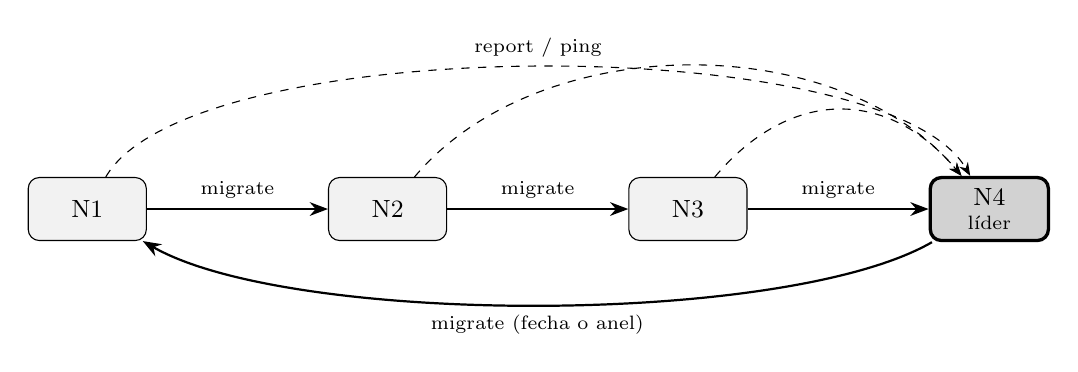
\begin{tikzpicture}[node distance=2.3cm, every node/.style={font=\small},
  n/.style={draw,rounded corners,minimum width=1.5cm,minimum height=0.8cm,align=center,fill=gray!10},
  l/.style={n,fill=gray!35,very thick}]
\node[n] (n1) {N1};
\node[n,right=of n1] (n2) {N2};
\node[n,right=of n2] (n3) {N3};
\node[l,right=of n3] (n4) {N4\\[-2pt]\scriptsize líder};
\draw[-{Stealth},thick] (n1)--node[above,font=\scriptsize]{migrate}(n2);
\draw[-{Stealth},thick] (n2)--node[above,font=\scriptsize]{migrate}(n3);
\draw[-{Stealth},thick] (n3)--node[above,font=\scriptsize]{migrate}(n4);
\draw[-{Stealth},thick] (n4) to[out=-150,in=-30,looseness=0.55] node[below,font=\scriptsize]{migrate (fecha o anel)} (n1);
\draw[-{Stealth},dashed] (n1) to[out=60,in=120,looseness=0.5] node[above,font=\scriptsize,pos=0.5]{report / ping} (n4);
\draw[-{Stealth},dashed] (n2) to[out=50,in=130,looseness=0.9] (n4);
\draw[-{Stealth},dashed] (n3) to[out=50,in=130,looseness=1.2] (n4);
\end{tikzpicture}
\caption{Topologia com 4 nós. Linhas cheias: migração em anel. Tracejadas: \code{report} e \code{ping} entre seguidores e líder. \code{election} e \code{coordinator} podem ser trocadas entre quaisquer nós.}
\label{fig:arq}
\end{figure}

\begin{table}[h]
\centering\small
\caption{Mensagens RPC. Toda chamada leva (remetente, timestamp de Lamport) e a resposta devolve o timestamp do respondente.}
\label{tab:msg}
\begin{tabular}{@{}lll@{}}
\toprule
Método & Trajeto & Conteúdo principal \\ \midrule
\code{ping} & líder $\leftrightarrow$ seguidores & vazio; resposta traz o líder conhecido \\
\code{election} & nó $\to$ IDs maiores & vazio; resposta \code{OK} \\
\code{coordinator} & novo líder $\to$ todos & anúncio; \code{REJECT} se receptor é maior \\
\code{migrate} & nó $\to$ vizinho no anel & $k$ melhores tours (listas de cidades) \\
\code{report} & nó $\to$ líder & geração, melhor tour/custo, \code{done} \\
\code{shutdown} & líder $\to$ todos & encerra o cluster \\ \bottomrule
\end{tabular}
\end{table}

\section{Implementação dos requisitos}
Atendemos três requisitos da lista do enunciado, todos implementados manualmente sobre o RPC.

\subsection{RPC}
Usamos o XML-RPC da biblioteca padrão do Python (o enunciado permite qualquer RPC; gRPC não estava disponível no ambiente de desenvolvimento e XML-RPC dispensa dependências). Cada nó expõe seis métodos. Do lado cliente, \code{Node.call} cria um proxy com \textit{timeout} (1 s), captura qualquer erro de rede e devolve \code{(ok, resultado)}, de modo que falhas de comunicação nunca derrubam o nó. Cada chamada incrementa em 1 o contador de falhas consecutivas do destino; três falhas o marcam como morto, e um sucesso zera o contador. Como todo RPC (migração, relatório, \textit{ping}) alimenta esse contador, a detecção ocorre rapidamente. O servidor atende cada requisição em uma thread própria.

\subsection{Relógios lógicos de Lamport}
Cada nó mantém um \code{LamportClock} protegido por \textit{lock}. Antes de enviar uma mensagem, o remetente executa $L \leftarrow L+1$ e anexa $L$; ao receber, o destinatário executa $L \leftarrow \max(L, t)+1$, e o mesmo vale para a resposta. Todos os eventos relevantes são registrados em log com o valor de $L$. Exemplo real: N1 enviou \code{migrate} com $t=5$; N2, cujo relógio estava em 11, passou para $\max(11,5)+1=12$. Os logs permitem verificar a relação \textit{aconteceu-antes} (um envio sempre tem $L$ menor que o recebimento correspondente). O relógio é usado para ordenar causalmente os eventos de eleição e migração na depuração, já que os relógios físicos das máquinas não são sincronizados.

\subsection{Eleição de líder (Bully)}
Cada nó possui um ID inteiro; vence o maior ID vivo. Um nó inicia a eleição ao subir ou ao detectar a queda do líder. Ele envia \code{election} a todos os IDs maiores. Se nenhum responde \code{OK}, ele se torna líder e envia \code{coordinator} a todos. Se algum responde, aguarda o anúncio por até 3 s e, se este não chegar, repete a eleição. Quem recebe \code{election} de um ID menor responde \code{OK} e inicia a própria eleição. Um \code{coordinator} vindo de ID menor é rejeitado, o que resolve a situação de dois líderes (por exemplo, quando um nó de ID alto volta). Seguidores fazem \textit{ping} ao líder a cada 1 s; o líder faz \textit{ping} a todos. Ao assumir, o novo líder zera a agregação, e os nós que já haviam terminado reenviam seu \code{report} final.

\subsection{Tolerância a falhas e término}
Se o vizinho do anel não responde, a migração tenta o próximo do anel. O líder só finaliza quando todos os nós \textit{vivos} informaram \code{done}; então grava o resultado (JSON) e envia \code{shutdown}.

\section{Resultados experimentais}
Os testes foram feitos em \textit{localhost}, com processos independentes, população total 240, 1500 gerações, 80 cidades e 3 sementes por configuração. A referência da heurística do vizinho mais próximo é 8406,7 (menor é melhor). A Tabela~\ref{tab:res} resume os resultados.

\begin{table}[h]
\centering\small
\caption{Comprimento do melhor tour (média e desvio padrão de 3 execuções).}
\label{tab:res}
\begin{tabular}{@{}lrr@{}}
\toprule
Configuração & Média & Desvio \\ \midrule
1 nó, população 240 & 9938,4 & 297,6 \\
1 nó isolado, população 60 (controle) & 7478,7 & 105,5 \\
2 nós $\times$ 120 & 7350,3 & 67,1 \\
4 nós $\times$ 60 & 7262,3 & 111,2 \\
5 nós $\times$ 48 & 7295,6 & 158,9 \\ \bottomrule
\end{tabular}
\end{table}

A maior parte da diferença entre o caso de 1 nó (população 240) e os demais se deve ao tamanho da subpopulação: com número fixo de gerações, populações menores convergem mais rápido, como mostra o controle de 1 nó com população 60. O efeito da migração isolado é modesto: 4 ilhas ficaram cerca de 3\% melhores que uma ilha isolada de mesmo tamanho. Com 5 nós o resultado não melhorou, indicando que ilhas pequenas demais perdem diversidade. Com três sementes, as diferenças entre 2, 4 e 5 nós estão dentro do desvio e não são conclusivas.

\textbf{Falhas injetadas} (4 nós, 3000 gerações): (i) ao matar o líder N4 aos $\sim$4 s, N3 detectou a falha em menos de 1 s, venceu a eleição e a execução terminou com tour 7003,9; (ii) ao matar o nó N2, N1 passou a migrar para N3 e a execução terminou com tour 7343,8. A população de um nó morto é perdida, pois não há \textit{checkpoint}.

\textbf{Limitação de medição:} o ambiente de teste tinha um único núcleo de CPU, portanto \textit{não medimos \textit{speedup}}; o \code{benchmark.py} deve ser executado em máquinas distintas da rede local para isso.

\section{Desafios e problemas encontrados}
\begin{itemize}
\item \textbf{Confundir efeito da distribuição com efeito do AG.} A comparação ingênua entre 1 nó e N nós superestimava o ganho; foi preciso um experimento de controle com mesma subpopulação.
\item \textbf{Concorrência.} Chamadas RPC chegam em threads diferentes da evolução; protegemos o relógio, a caixa de imigrantes e o estado de agregação com \textit{locks}, e evitamos eleições simultâneas com uma \textit{flag} sob \textit{lock}.
\item \textbf{Detecção de falhas e tempestade de eleições.} Na partida, todos os nós iniciam eleição ao mesmo tempo; a \textit{flag} de eleição em andamento e o \code{REJECT} evitam múltiplos líderes.
\item \textbf{Término com falhas.} O líder precisa saber quem ainda está vivo para não esperar eternamente; isso exigiu o contador de falhas e o reenvio do \code{report} final após troca de líder.
\item \textbf{Ambiente.} gRPC não estava disponível sem rede, o que motivou o XML-RPC; os \textit{timeouts} exigiram um \textit{transport} próprio.
\end{itemize}

\section{Papel de cada aluno}
\begin{itemize}
\item \textbf{Aluno 1:} arquitetura, protocolo de mensagens e camada RPC (\code{rpc.py}, \code{Node.call}), \textit{timeouts} e tratamento de falhas de comunicação.
\item \textbf{Aluno 2:} eleição Bully, \textit{heartbeat} e detecção de falha do líder.
\item \textbf{Aluno 3:} relógio de Lamport, integração nas mensagens e formato dos logs.
\item \textbf{Aluno 4:} algoritmo genético (TSP, OX, mutação, seleção), ilhas e política de migração.
\item \textbf{Aluno 5:} \code{run\_local.py}, \code{benchmark.py}, injeção de falhas, experimentos, README e relatório.
\end{itemize}
O código está disponível no projeto entregue, com instruções no \code{README.md}.

\end{document}
